%!TEX root = ../../../FYP_Dissertation.tex

In this section we present another case of surprising performance of MAD that
ended up being also attributed to the object model. In this example we are going
to talk about the iterator of the \emph{Sequence} data-structure.

To recall,
\emph{Sequence} is used to represent particle accelerator by composition of
different Elements. In addition of the index, and the actual element the iterator
return its \emph{spos} (distance in meters from the start of the sequence). The
only difference between forward and backward iterators is that for forward iterator
the \emph{spos} is precomputed for each elements and stored in a table while for
backward we need to take the \emph{spos} of the element and add its length. This
makes the difference of performance relying only on the access of the length of
an element and a simple addition.

The code below shows the two examples that we are comparing. We iterate in each
case 20000 times over the \emph{LHCB1} sequence (a circular accelerator) with
the first case using the forward iterator and the second case using the backward
iterator (iterate from the end of the sequence to the beginning).

Figure \ref{fig:MO-seq-iter-curve}, shows the performance of ten independent
runs of the two cases. The forward iterator take around 0.3 seconds when the
backward one takes around 30 seconds to complete. The first natural things to do
to try to understand why is to study the trace dump. Figure \ref{fig:MO-seq-iter},
shows a screenshot of the generated dump files and we can clearly this that
something is wrong as it generates files over 300 times heavier.

Indeed the simplest examples explored in Section \ref{Sec:MO-perf-analys} doesn't
show what happens when each object that we query store the requested variable at
a different hierarchy depth. This is exactly what we have here, Figure
\ref{fig:MO-seq-iter-schematic} illustrates how the different elements that
constitute a sequence might look like. The requested \emph{l} value (the length
of the corresponding element) might be stored at a different depth depending on
the nature of the element. Since the hierarchical lookup is completely inlined
in the trace, we end up needing to generate a different set of traces for each
depth.

A potential quick fix for this particular case would be to also store the
backward \emph{spos} in a table during the \emph{Sequence} construction.

\begin{lstlisting}[style=LuaStyle]
-- load LHC 1st beam sequence
local lhcb1 = loadLHC()

local cnt = 0

-- 1st case : forward iterator
for i, elem, s in lhcb1:iter(nil, 2e4, 1) do
	cnt = cnt + i
end

-- 2nd case : backward iterator (negative direction)
for i, elem, s in lhcb1:iter(nil, 2e4, -1) do
	cnt = cnt + i
end
\end{lstlisting}

\begin{figure}[H]
    \centering
    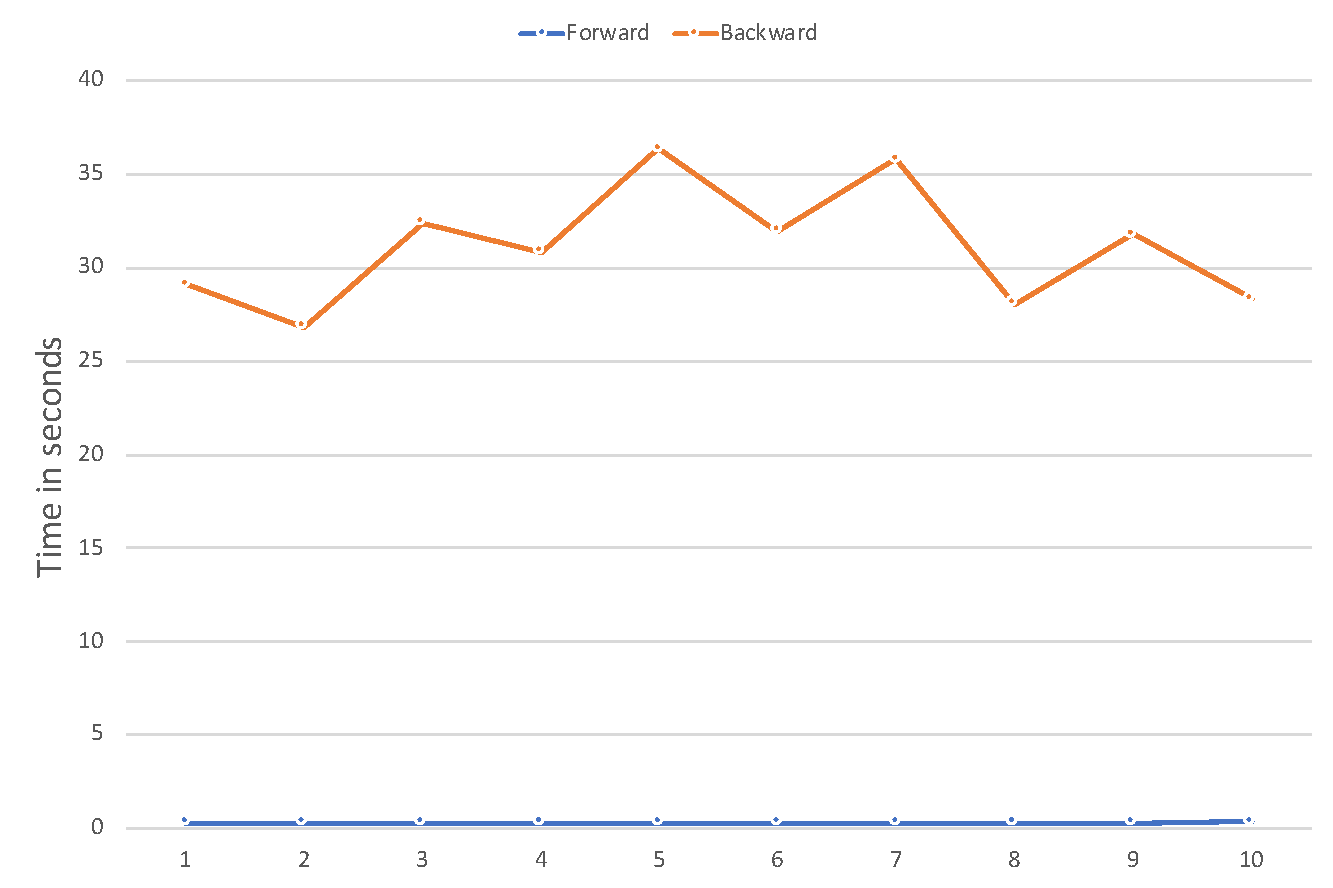
\includegraphics[width=0.8\textwidth]{./Images/seq-iter-curve.pdf}
    \caption{Multiple runs of each cases presented above}
    \label{fig:MO-seq-iter-curve}
\end{figure}

\begin{figure}[H]
    \centering
    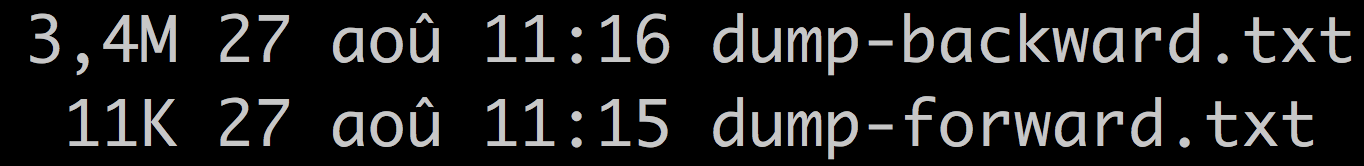
\includegraphics[width=0.6\textwidth]{./Images/dump-size}
    \caption{Screenshot of the size of the dump file for those two cases}
    \label{fig:MO-seq-iter}
\end{figure}

\begin{figure}[H]
    \centering
    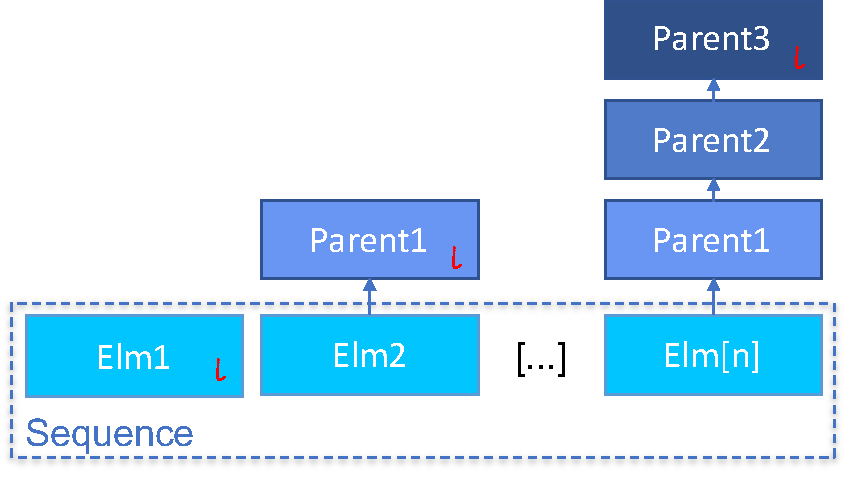
\includegraphics[width=0.8\textwidth]{./Images/seq-iter-schematic.pdf}
    \caption{Illustration of the \emph{Sequence} in this example}
    \label{fig:MO-seq-iter-schematic}
\end{figure}
